% 2008 年上海卷文科第 16 题：棱长 2 的正方体 ABCD-A1B1C1D1，E 为 BC1 的中点，
%   求直线 DE 与平面 ABCD 所成的角。
% 来源 PDF：gaokaomath-src/普通高考/2008/2008上海文.pdf
% SHA-256：415d384fcd05cab11debea2d8a328f9daf1d1880ffd26c915df999f7bae589a4
% 原页：2008上海文.pdf 第 1 页（A3 三栏）第 2 栏，书页码 481。
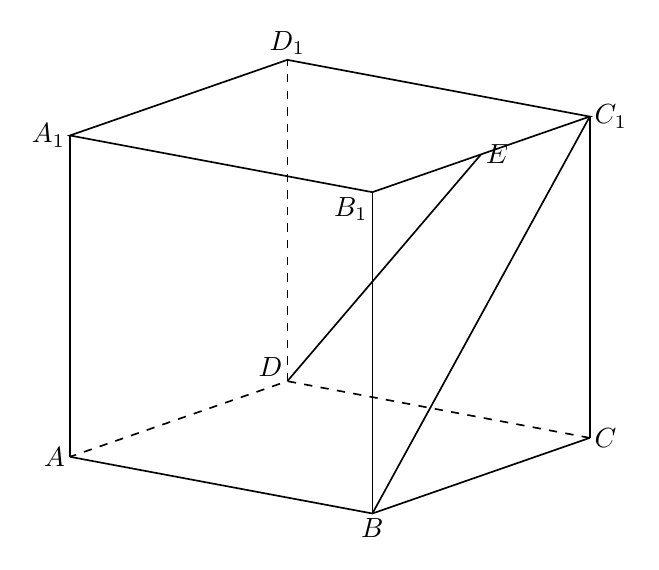
\begin{tikzpicture}[scale=1.2, semithick,
  every node/.style={inner sep=1.5pt}]
  \coordinate (A)  at (0.0,0.9);
  \coordinate (B)  at (3.2,0.3);
  \coordinate (C)  at (5.5,1.1);
  \coordinate (D)  at (2.3,1.7);
  \coordinate (A1) at (0.0,4.3);
  \coordinate (B1) at (3.2,3.7);
  \coordinate (C1) at (5.5,4.5);
  \coordinate (D1) at (2.3,5.1);
  \coordinate (E)  at (4.35,4.1);

  \draw (A) -- (B) -- (C);
  \draw[dashed] (C) -- (D) -- (A);
  \draw (A) -- (A1);
  \draw (B) -- (B1);
  \draw (C) -- (C1);
  \draw (D1) -- (A1) -- (B1) -- (C1) -- cycle;
  \draw[dashed] (D) -- (D1);

  \draw (D) -- (E);
  \draw (B) -- (C1);

  \node[left] at (A) {$A$};
  \node[below] at (B) {$B$};
  \node[right] at (C) {$C$};
  \node[above left] at (D) {$D$};
  \node[left] at (A1) {$A_1$};
  \node[below left] at (B1) {$B_1$};
  \node[right] at (C1) {$C_1$};
  \node[above] at (D1) {$D_1$};
  \node[right] at (E) {$E$};
\end{tikzpicture}
